% This is LLNCS.DEM the demonstration file of
% the LaTeX macro package from Springer-Verlag
% for Lecture Notes in Computer Science,
% version 2.4 for LaTeX2e as of 16. April 2010
%
\documentclass{llncs}
%
% \usepackage{natbib}
\usepackage{CJK}
\begin{CJK}{UTF8}{song}
\usepackage{makeidx}  % allows for indexgeneration
\usepackage{graphicx}
\usepackage{epstopdf}
\usepackage{subfigure}
\usepackage{booktabs}
\usepackage{color}

\begin{document}

\title{An Approach for the Chinese Question-answer System based on Document}
%
\titlerunning{Chinese Question-answer System}  % abbreviated title (for running head)
%                                     also used for the TOC unless
%                                     \toctitle is used
%
\author{Benyou Wang\inst{1} \and Jiabing Niu\inst{1} \and Liqun Ma\inst{1} \and Yuhua Zhang\inst{1} \and Lipeng Zhang\inst{1}
\and Peng Zhang\inst{1}}
%
\authorrunning{Benyou Wang et al.} % abbreviated author list (for running head)
%
%%%% list of authors for the TOC (use if author list has to be modified)
\tocauthor{Benyou Wang, Jiabing Niu, Liqun Ma, Yuhua Zhang, Lipeng Zhang
, and Peng Zhang}
%
\institute{%
Tianjin Key Laboratory of Cognitive Computing and Application, School of Computer Science and Technology, Tianjin University, Tianjin, China\\
% \and Computing and Communications Department, The Open University, United Kingdom \\
% \and Department of Information Engineering, University of Padua, Italy
}


\maketitle              % typeset the title of the contribution



\begin{abstract}
Question Answering system has gradually become a new trend within the field of information retrieval and NLP. It outperforms the conventional search engines, for the system is able to answer users’ questions automatically and accurately. Question Answering system based on English corpus has developed rapidly, whereas the Chinese corpus based Question Answering system still has some problems remains to be solved. Thus, developing a new Question Answering model, which is characterized by dealing with features of Chinese corpus is extemely essentail. Different to the current deep learning model, our model uses the semantic and syntactic information in Chinese corpus and bases on the linearity of Chinese texts. Finally, our model turns out to perform better than other methods through experiments.\dots
\keywords{Question Answer, DBQA, semantic matching, Chinese QA}
\end{abstract}
%
\section{Introduction}

Quesion Answering (QA) have {\color{red} attracted great}  attention with the development of Natural Language Processing and Information Retrieval techniques. One of the typical tasks named document-based quetion answer (DBQA) concentrates on finding the answers from the question's given documents.
Comparing to the tranditional document retrieval task, DBQA system usually use fluent natural language to express the query intent and  {\color{red}an} accurate result  {\color{red}which has discarded most} unmatching candidates is needed. 

Due to the shorter text in QA task, the term independency hypothesis and data sparsity  {\color{red}have become} more serious problems than  {\color{red}those of}the tranditional retrieval task. The relevance-based IR methods like TFIDF or BM-25 cannot solve  {\color{red}these} precise matching problems {\color{red}properly}. Thus, word embedding technology \cite{Mikolov2013Efficient} is  {\color{red}inclined} to  {\color{red}be} widely applied in some English QA system as well as the Chinese QA system. Moreover, the question text is natural language with complete syntax structures instead of some keywords in document-retrieve task. The sentence of a question should be considered as a sequence structure or a tree structure, which can {\color{red}be paid} different attention on different parts. In summary, a QA system should consider {\color{red}the following} problems simultaneously.

1) match the semantics-similar texts which may be synonymous paraphrased.  

2) take the sequantial information of the question text into consideration, instead of an unordered set of words.

For the first problem, enumerating all the paraphrase rules of English or Chinese seems to be impossible. When we adopt the distributed representation, two words which {\color{red}are} similar in semantics may have a closed embedding representations. {\color{red}Given} the term independency hypothesis, for a query \emph{a cute pet}, \emph{a dog} or \emph{a cat} cannot be found in the return list, but the embedding-based method can. In Chinese, many similar words may share the same character based on the specific word formation of Chinese. For exmaple, the two words ``表演'' or ``演出'' have the same meaning as ``perform or show'' in English. Some character-based technology may help a lot.  
{\color{red}According to} the Chinese expression habit, people are more likely to firstly elaborate the premise and then ask the related issues under such premise. In the bag-of-words model, an unordered set of words in questions will lose the information to distinguish the premise and issues and {\color{red}the focuses} on the issues.

This paper {\color{red}elaborates} an approach for the Open Domain Questin Answering shared sub-task of Document-based QA task in NLPCC-ICCPOL 2016. We conbine the count-based method and embedding-base method with {\color{red}an} ensemble learning strategy. In order to adapt to the Chinese expression habit, we integrate the features of Chinese into both the count-based method and embedding-based method, which achieves significant improvement upon baselines in the final evaluation.

%Conventional search engines, such as bing, Google and Baidu, are keywords based systems which are able to return a large number of results containing hyperlinks related to keywords in users' queries. However, users usually have to browse dozens of results to find their target answers if the first few results couldn't meet their needs. Therefore, question answering system is designed to answer users' short question sentences as well as combined phrases directly and accurately, for only one exact answer will be returned by the question anwsering system, which outperforms the conventinal search engines to some degree. Meanwhile, there are still some difficulties remain to be solved in the Chinese corpus based question answering system compared with the English corpus based one. For example, 中文QA的难点。词向量独立性假设。

The aim of the task is to build a system {\color{red}to select} the answers of thousands of questions. The target answers are only supposed to be selected from the question's given document {\color{red}which} contains a set of answer sentences. 
The results will finally be evaluated by the evaluation metrics to figure out the performance of our system. 
For example, for the given question ``俄罗斯贝加尔湖的面积有多大?'' in training set, the participants should find the correct answer ``贝加尔湖长636公里,平均宽48公里,最宽79.4公里,面积3.15万平方公里'' from the candidate answers. The model should generate a set of relevance scores between the question and each answer sentence including the correct answer in the test set. The evaluation toolkit which has test sets labeled golden answer annotations to questions will rank all answer sentences according to MRR scores and MAP scores. 
%And finally give the MRR and MAP value of our model as the evaluation metrics.

% We propose a method which integrates various features extracted from the question and answer sentences to form a model, which makes full use of the semantic and syntactic information as well as the linearity of Chinese corpus. 方法模型介绍. And our model outperforms other models including deep learning model according to the  experimental results.

The structure of this paper can be listed as follows. Sec.~\ref{sec:methods} introduces the methods including features and model which we use to complete the shared task. Sec.~\ref{sec:results}  presents the experiments and results we get. Sec.~\ref{sec:discussion} are discussions and conclutions.

\section{Related Work}

QA task focuses on automatically {\color{red}understanding} natural language questions and {\color{red}selecting} or {\color{red}generating} one answer (or more) which can match  the question semantically. %In the English QA system based on document, many efforts have been made to achieve a continually  better performance. 
Due to the shorter text than {\color{red}that of} the tranditional task of document retrieval, structured semantic information and  the lexical gap are two key points for QA system. 
For the first point, tree \cite{Yao2013Answer} or sequential \cite{Wang2015FAQ} structure have been proposed to utilize the syntactic information instead of an  unorderd bag-of-word model.
Some efforts like lexical semantics \cite{Yih2013Question}, probabilistic paraphrase or translation \cite{Zhou2011Phrase} have been made to alleviate the problem of lexical gap.
Moreover, feature-based ensemble method \cite{Severyn2013Automatic} try to combines both the semantic and syntactic information to rank the answers. Recently, the end-to-end strategy motivates us to build a deep symantic matching model which can also model the sequential text. With the development of the embedding-based neural network, deep {\color{red}learning} \cite{Yu2014Deep} \cite{Feng2015Applying} has achieved a good performance in the QA task. Severyn et.al. proposes a shallow convolutional neural network (CNN) which combines the ordered overlapped information into the hidden layer~\cite{severyn2015learning}. Recurrent neural network(RNN) and the following long short-term memory neural network (LSTM) \cite{Wang2015A} \cite{Tan2015LSTM} which can model the sequential text is also applicable for the represention and matching of quetion and answers. Santos et.al. proposes an attentive pooling networks with two-way attention mechanism for modelling the interactions between two sequential text and  integrating a CNN or RNN network easily~\cite{Santos2016Attentive}.
In Chinese, we need a more 


中文QA 的发展
我们的方法


\section{Methods}
\label{sec:methods}
%\subsection{Data Exploration}
We adopt a classical process for a competition task, with the successive steps from data exploration (in Sec~\ref{sec:exploration}), data preprocess (in Sec~\ref{sec:preprocess}), feature extraction (in Sec~\ref{sec:feature}) to model selection (in Sec~\ref{sec:model}).

\subsection{Data Exploration}
\label{sec:exploration}

In this section, we will {\color{red}explore} the characters of the train data and test data.
\subsubsection{basic statistics}
There are 181882 quetion-answer pairs with 8772 questions in the training set, and 122532 question-answer pairs with 5779 questions in the testing set. Every question have 20 candidate answers in the training set and 21 candidate answers in the testing set.

\begin{table}[!hbp]
\caption{the basic information of the training and testing set.}
\small % Font size can be changed to match table content. Recommend 10 pt by default.
\centering
\begin{tabular}{{p{6.5cm}p{3cm}p{3cm}}}
\toprule
\textbf{}	& \textbf{training set}	& \textbf{testing set}\\
\midrule
number of qa pairs & 181882 & 122532  \\
number of questions & 8772 & 5779 \\
average number of candidate answer & 20.7 & 21.2 \\
average length of the questions (charater) & 46.3 & 46.2 \\
average length of the answers (charater) & 106.0 & 106.5 \\
average number of correct answers & 1.05 & 1.06 \\

\bottomrule
\end{tabular}
\label{fig:basicinfo}
\end{table}

\subsubsection{question types}

Different questions will have different information need. Question sentences’ type is usually a kind of vital signal. It is a prerequisite but not sufficient condition when distinguishing whether the given sentence is a correct answer or not. For example {\color{red}for} the question ``中央大学的首任校长是谁?'', a candidate answer can be correct only if  it appears a name entity of person.
%Sometimes we can only infer that which kind of answer have the probability to becoming the correct answers. For examples, you want get the name of somebody or a number of some count-based events.
We divide the question into the following categories:

\begin{table}[!hbp]
\caption{the number of different types of question.}
\small % Font size can be changed to match table content. Recommend 10 pt by default.
\centering
\begin{tabular}{{p{6.5cm}p{3cm}p{3cm}}}
\toprule
\textbf{}	& \textbf{training set}	& \textbf{testing set}\\
\midrule
time & 950 & 861  \\
number & 2135 & 1433 \\
person name & 1049 & 526 \\
place name & 583 &  396\\
organazation name & 185 & 137 \\
others & 3870 & 2646 \\
{\color{red}total} & & \\
\bottomrule
\end{tabular}
\label{fig:typeinfo}
\end{table}





\subsubsection{word-level and character-level overlap}

For a question like ``佛罗伦萨什么时候降水比较多?'', the unique answer ``降水主要集中在冬季'' will share the same component ``降水''. {\color{red}For} most Chinese word segmentation tools, ``降水'' can be
segmented as a single word, which is usually considered as the minimal granularity of semantic units. Except for some paraphrased cases, the answer will cover the issues of the question by overlapping some words with the question. In the whole training test, we get the trend as showed in the Fig.~\ref{fig:word_overlap}. It is easily found in the range from 0 to 13 of the x-axis, the more overlapped words between the question-answer pairs, the more likely the pairs match. Moreover, the information of character-level overlap will cover many paraphrased patterns of Chinese. For example {\color{red}for} the question ``“年”字有多少笔?'', the correct answer ``笔划:6'' {\color{red}has} three words [``笔划'',``:'',``6''] and does not have any overlapped words with the question.  Fig.~\ref{fig:character_overlap} shows {\color{red}that} the word-level overlap has the similar trend to be the correct answers. 


%\includegraphics[width=3in]{sensitive_simple_trec2013.pdf}

\begin{figure}[htb]
	\begin{minipage}[t]{0.5\linewidth} 
	\subfigure

		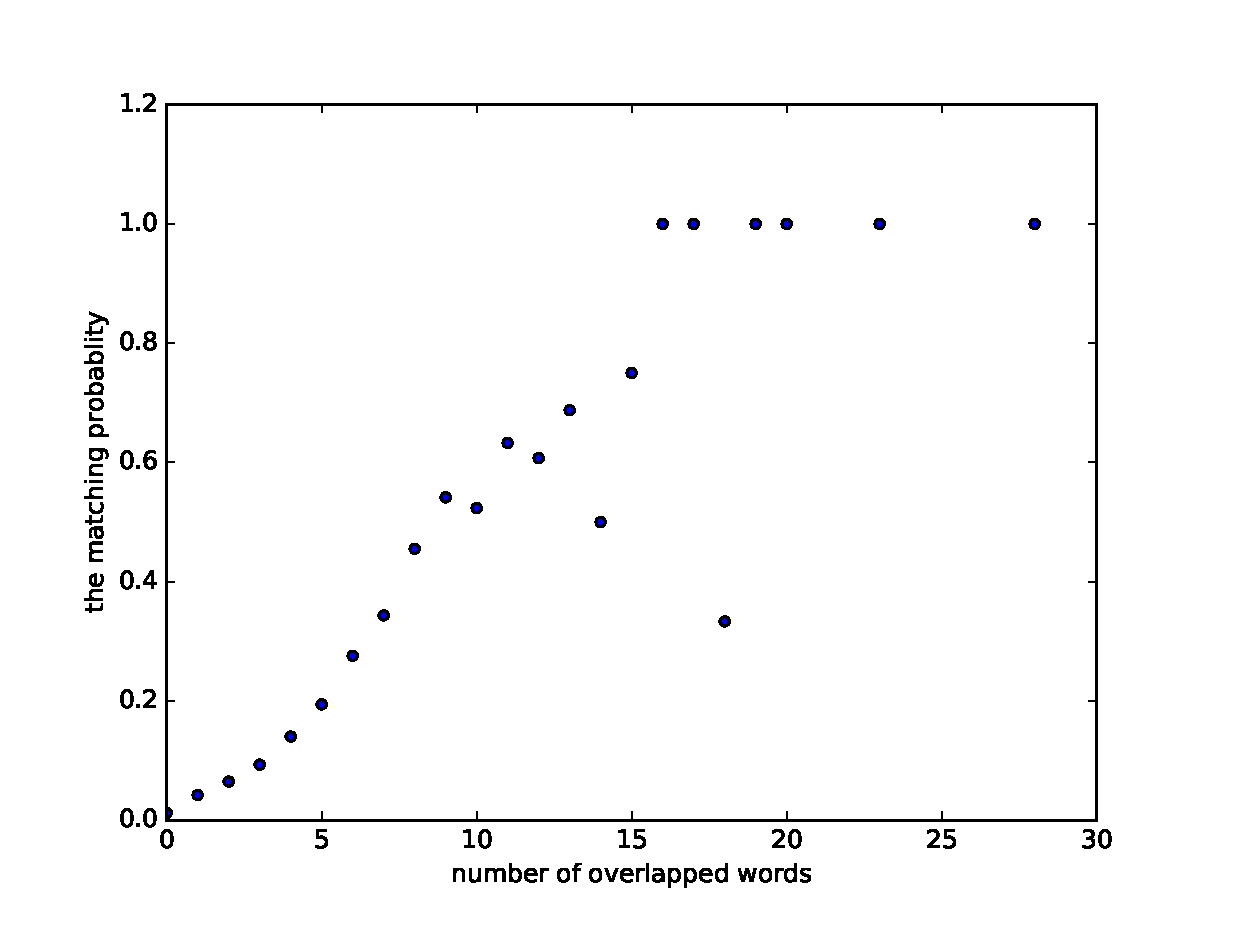
\includegraphics[width=2.5in]{figures/word_overlap.eps}
		\caption{x-axis means the number of overlapped words in both question and answer sentences. y-axis refers to the probable occurrence frequency of the target answer. Data scatters after the number of 14 for the lack of words samples.}
		\label{fig:word_overlap}
	\end{minipage}
	\hspace{1ex} 
	\begin{minipage}[t]{0.5\linewidth} 
	\subfigure
	\centering
		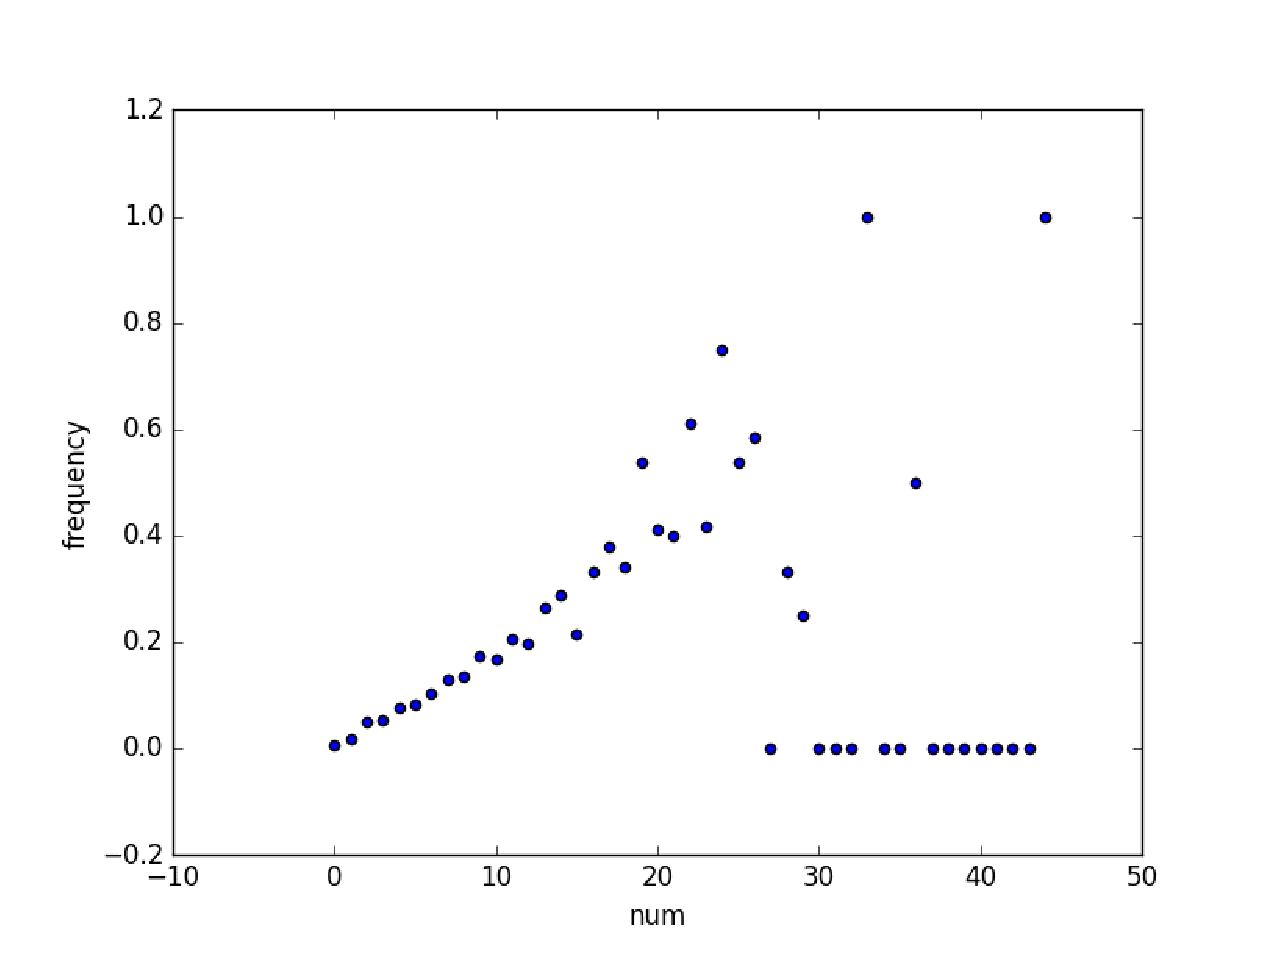
\includegraphics[width=2.5in]{figures/character_overlap.eps}
		\caption{x-axis means the number of overlapped characters in both question and answer sentences. While y-axis refers to the probability of becoming the target answer. Data are dispersed in the range between 22 and 50 because the samples are not enough.}
		\label{fig:character_overlap}
	\end{minipage}
\end{figure}

% We first segment the question and answer sentences into a series of characters and then count the total overlapped chatacers between the question and answer characters.As what has been shown in Fig. \ref{fig:character_overlap},it is concluded that there is a linear dependence between the correct answers’ frequency and overlapped characters.The same methods are also applied to the overlapped words and Fig. \ref{fig:word_overlap} illustrates that the more words are overlapped,the more likely that the answer is the correct one.

\subsubsection{Sequential structure informations}

Tranditional IR model like TF-IDF or BM25 model treats a query or a document as a bag of words, in which the sequential information of structure are ignored. In the scenario of QA system with a shorter length of question and answer, sequential information may help a lot for the matching of the question-answer pairs and a more elaborate model which takes the sequential information into consideration is needed. Roughly speaking, the word in different {\color{red}position} of a sentence may reflect different syntactic and semantic structures. For the example of the question ``中央大学的首任校长是谁?'', the word ``中央大学'' in the forward position is the limited premise of the issues of the latter words ``首任校长''.  The rearward word ``首任校长'' may be more related to the issues, which will contribute more to question-answer matching. In the training and testing set, we find the statistical correlation between the overlapped position and its corresponding probability of question-answer matching in Fig.~\ref{fig:word_position} for word-level overlap and Fig.~\ref{fig:word_position} for character-level overlap. 



%In Chinese grammer, different grammatical elements are usually distributed in different position in a sentence. For example, in a classic question, the entities concerned usually turn up in the front of a sentence, which follows the interrogatives like ,”什么?几个?多少?”.People have various speaking habits when they organize a sentence in Chinese.For instance, premises are more inclined to appear first in one sentence.So it is reasonable to consider keywords’ position message when we are trying to get the degree of how question and answer matches. We try to give different weights to keywords in different positions in a sentence.Meanwhile, weights may also be concerned with words’ idf values, which means the discrimination of words.
\begin{figure}[htb]
	\begin{minipage}[t]{0.5\linewidth} 
	\subfigure

		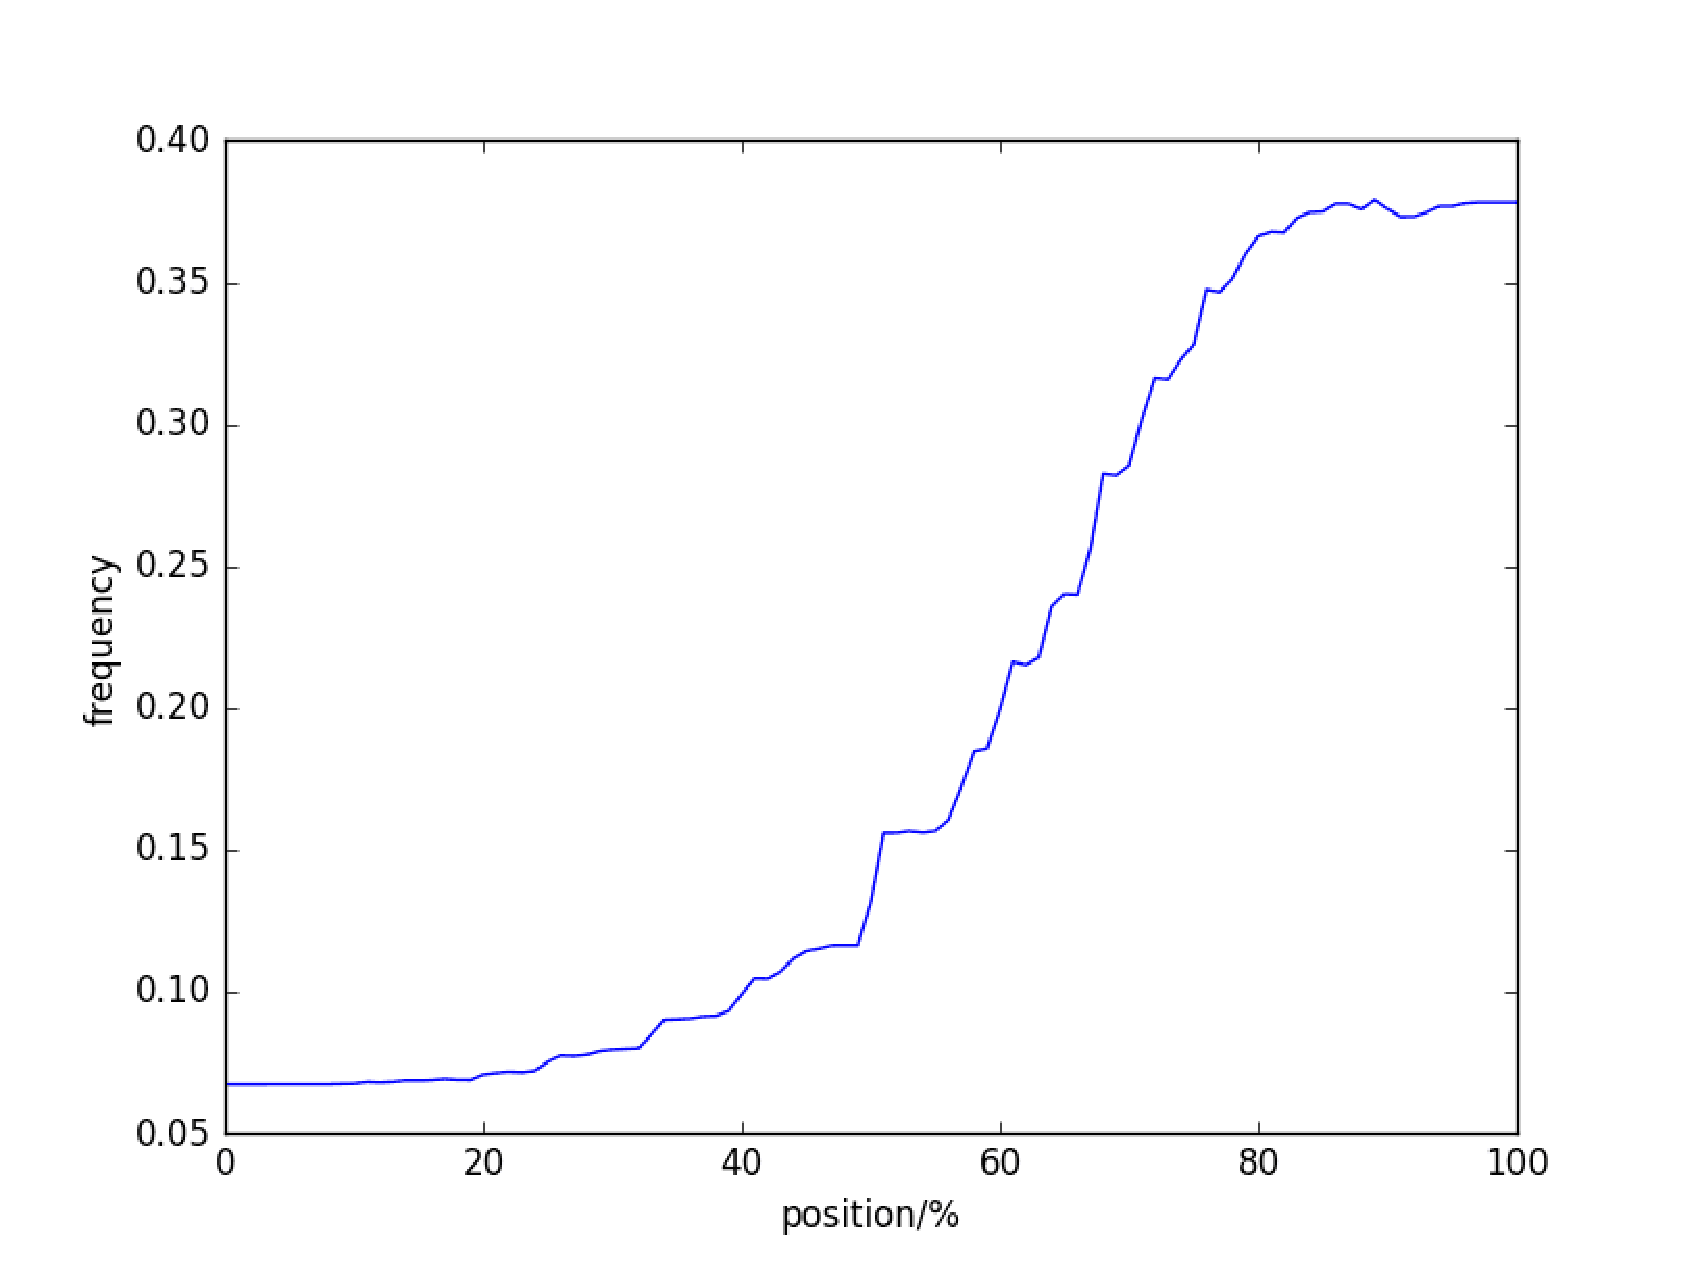
\includegraphics[width=2.5in]{figures/word_position.eps}
		\caption{x-axis refers to the position of the overlapped characters in question sentences. x=0 means that the overlapped character is on the front of  a sentence.x=100\% means the overlapped character is on the back of a sentence.y-axis means the occurrence frenquency of correct answers.}
		\label{fig:character_position}
	\end{minipage}
	\hspace{1ex}  
	\begin{minipage}[t]{0.5\linewidth} 
	\subfigure
	\centering
		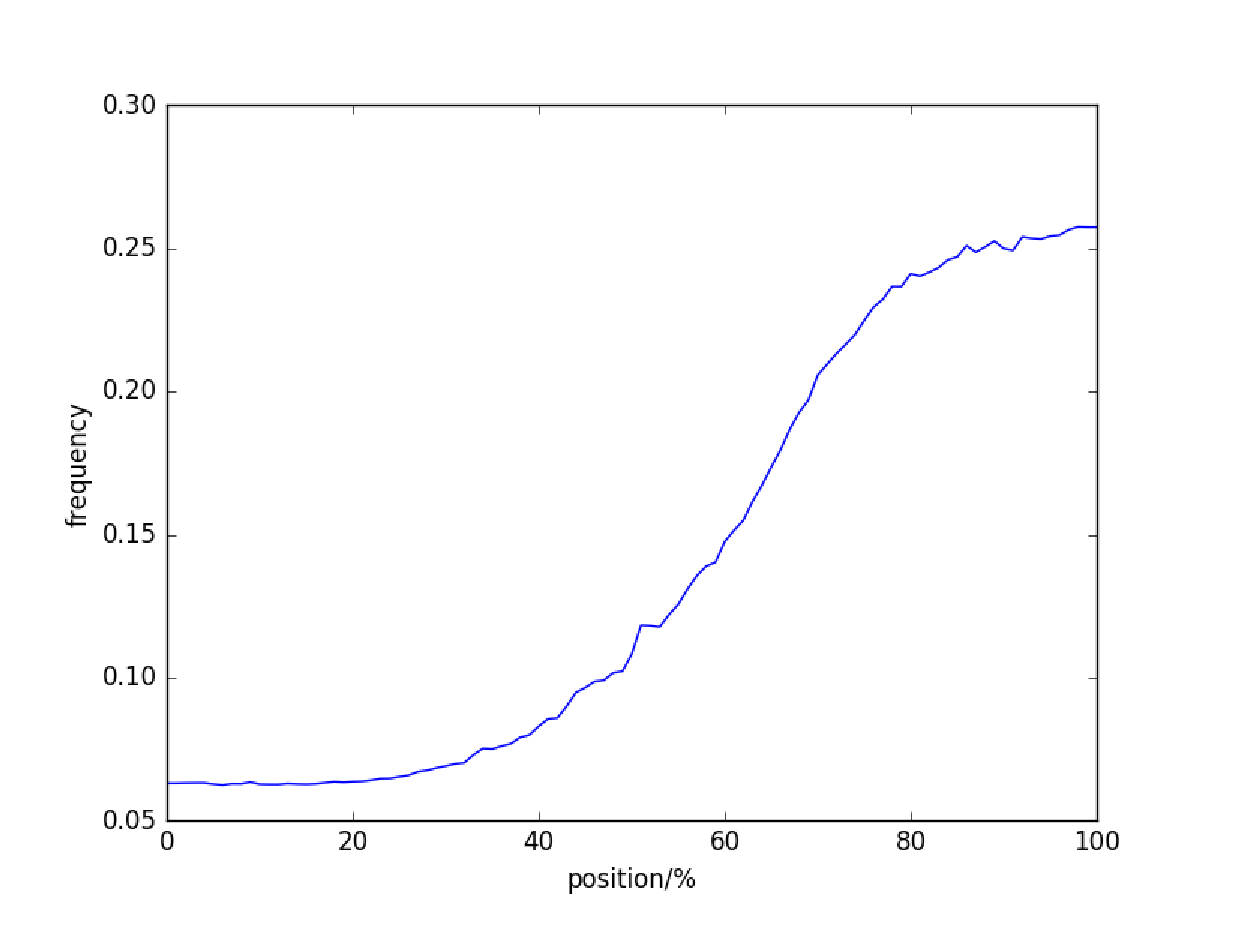
\includegraphics[width=2.5in]{figures/character_position.eps}
		\caption{Similar to Fig.~\ref{fig:character_position}, this figure shows the relationship between the position of the overlapped words in question sentences and the occurrence frenquency of correct answers.}
		\label{fig:word_position}
	\end{minipage} 
\end{figure}






% \begin{figure}[H]  
% \begin{minipage}[t]{0.5\linewidth} 
%  \centering  
%  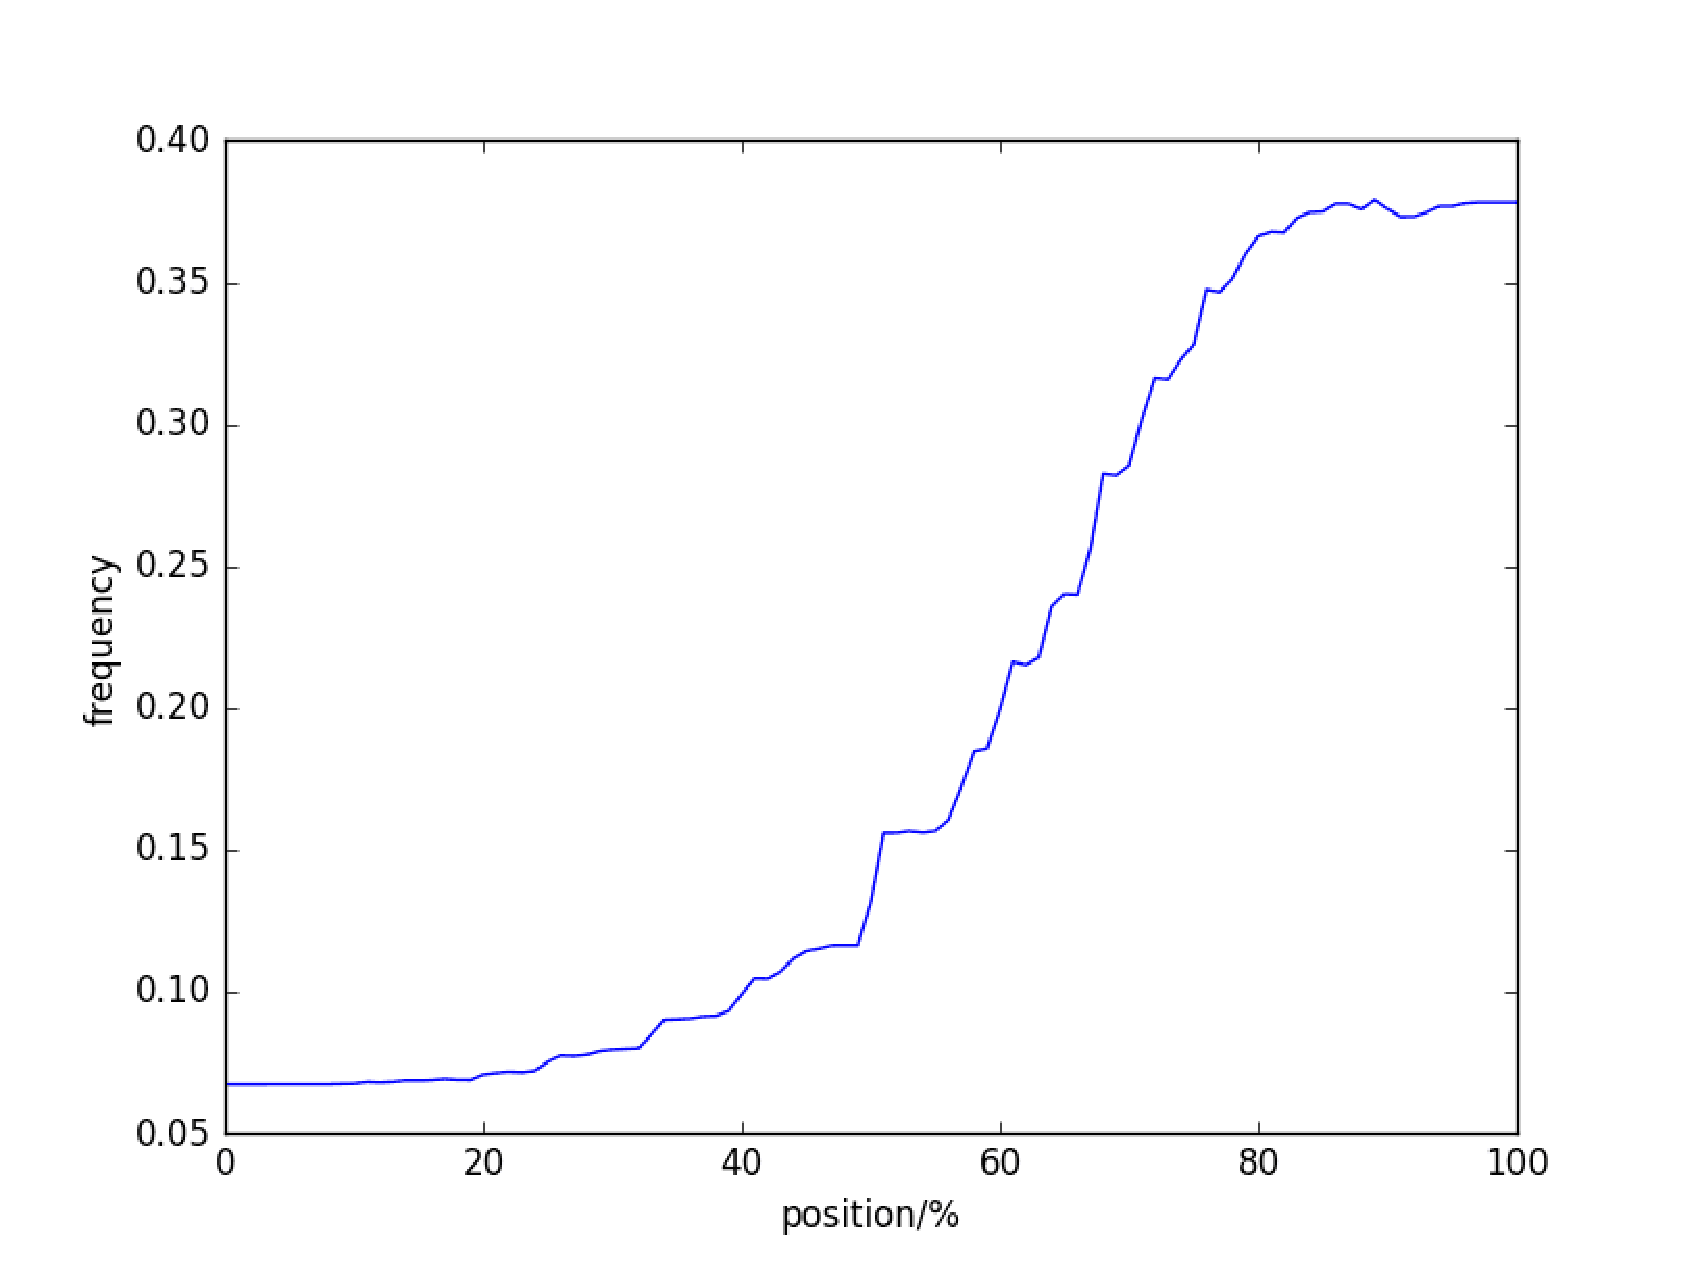
\includegraphics[width=8 cm]{figures/word_position.eps} 
%  \caption{Feasible rescheduled timetable II} 
%  \label{fig_pre-specified_sample} 
%  \end{minipage}
%   \hspace{1ex}  
%   \begin{minipage}[t]{0.5\linewidth} 
%   \centering  
%   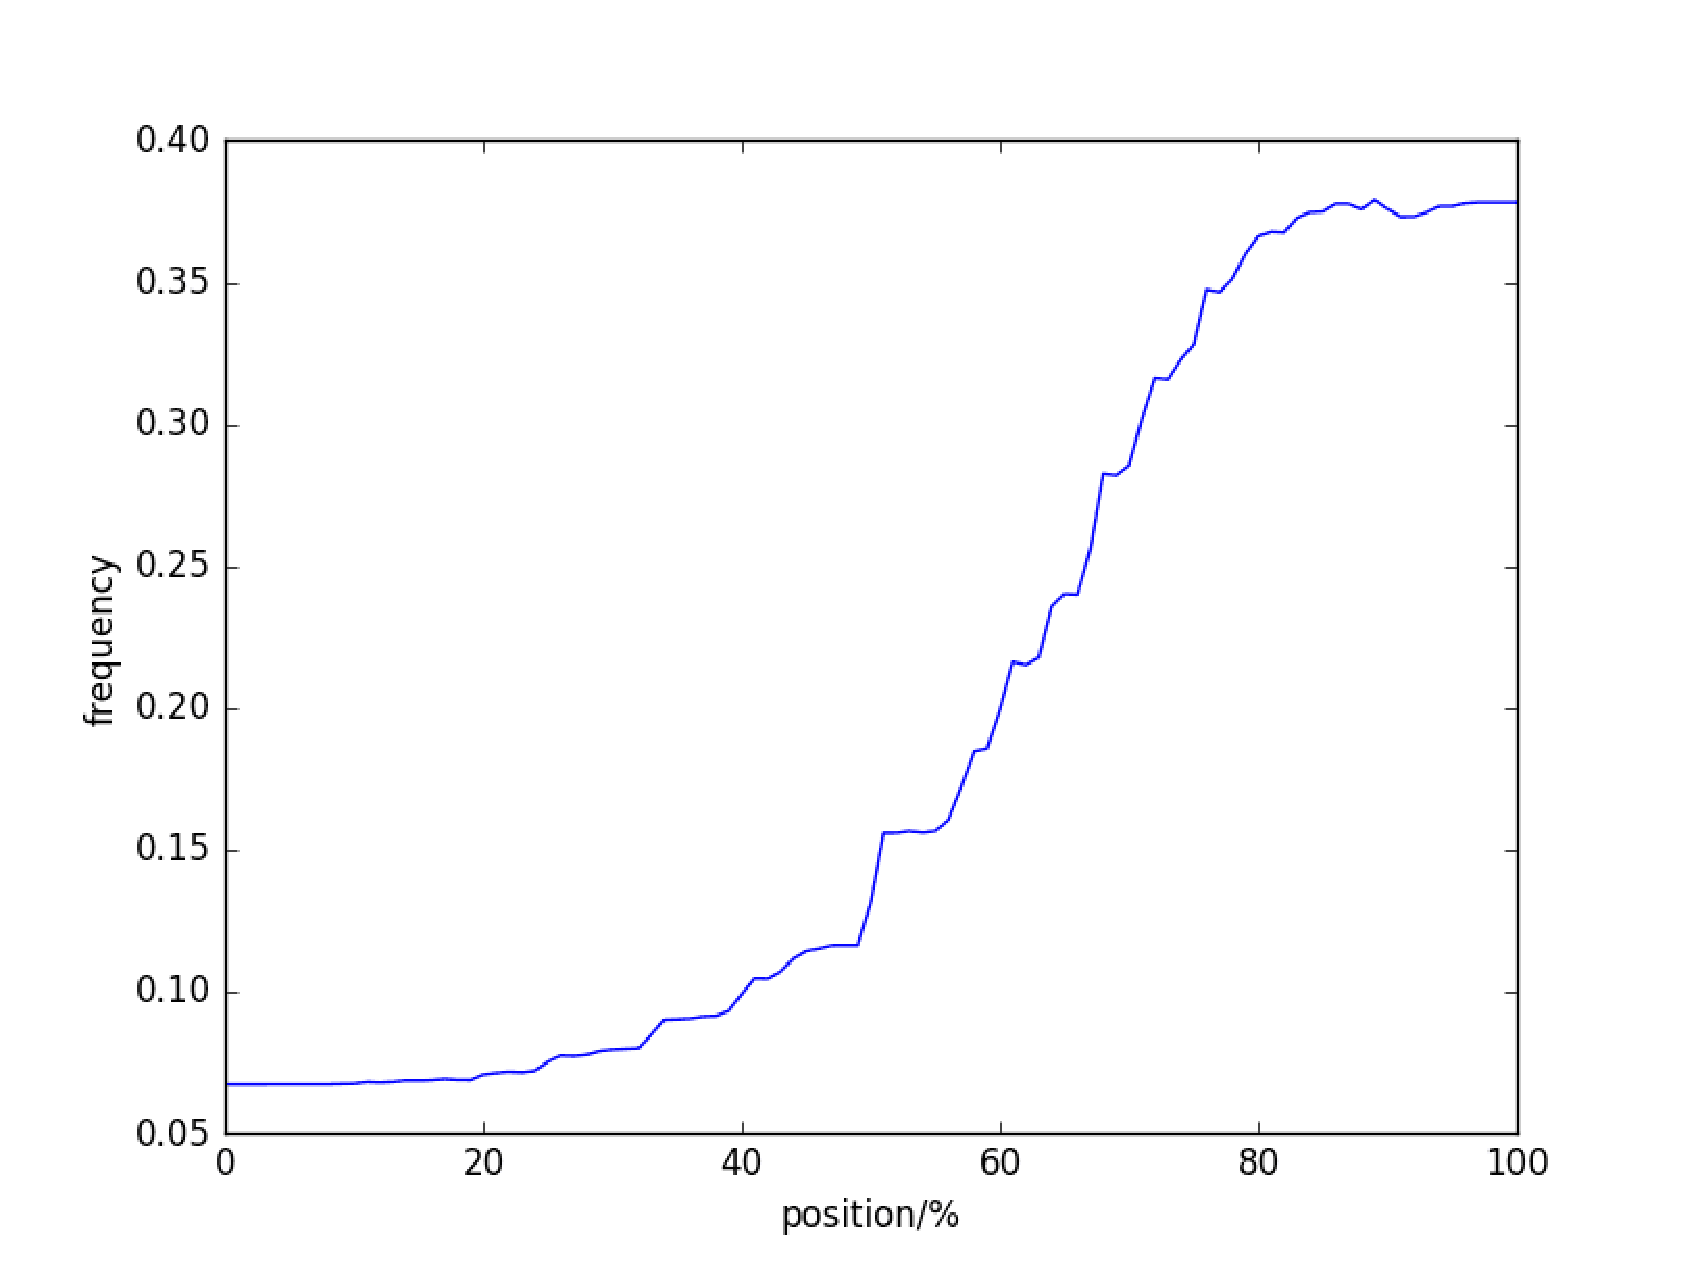
\includegraphics[width=8 cm]{figures/word_position.eps} 
%   \caption{Feasible rescheduled timetable I} 
%   \label{fig_rescheduled-timetable_sample} 
%   \end{minipage} 
%   \end{figure} 



% \begin{figure}[htb]
% \subfigure
% 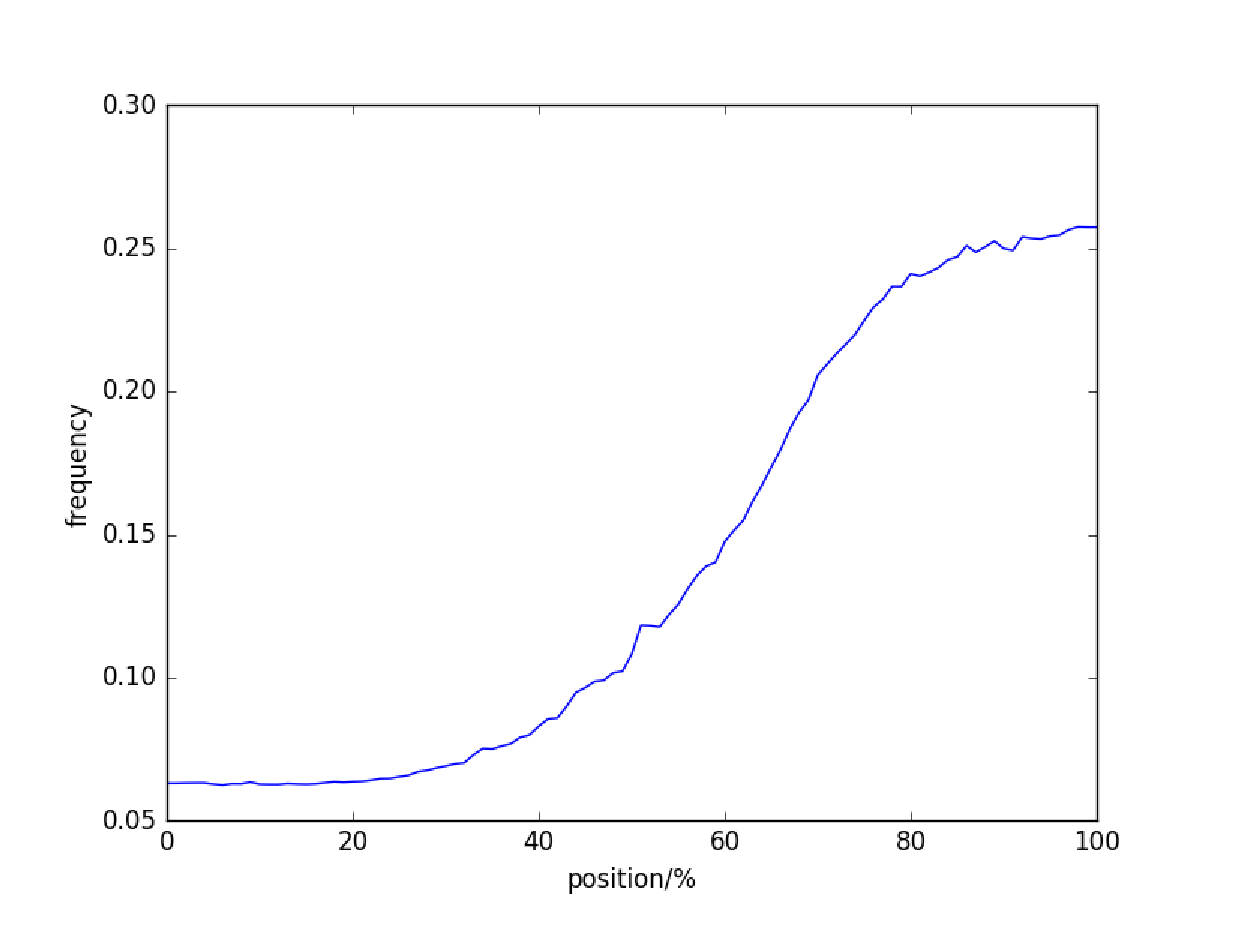
\includegraphics[width=2in]{figures/character_position.eps}
% \caption{x-axis refers to the position of the overlapped characters in question sentences. x=0 means that the overlapped character is on the front of  a sentence.x=100\% means the overlapped character is on the back of a sentence.y-axis means the occurrence frenquency of correct answers.}
% \label{fig:character_position}
% \subfigure
% 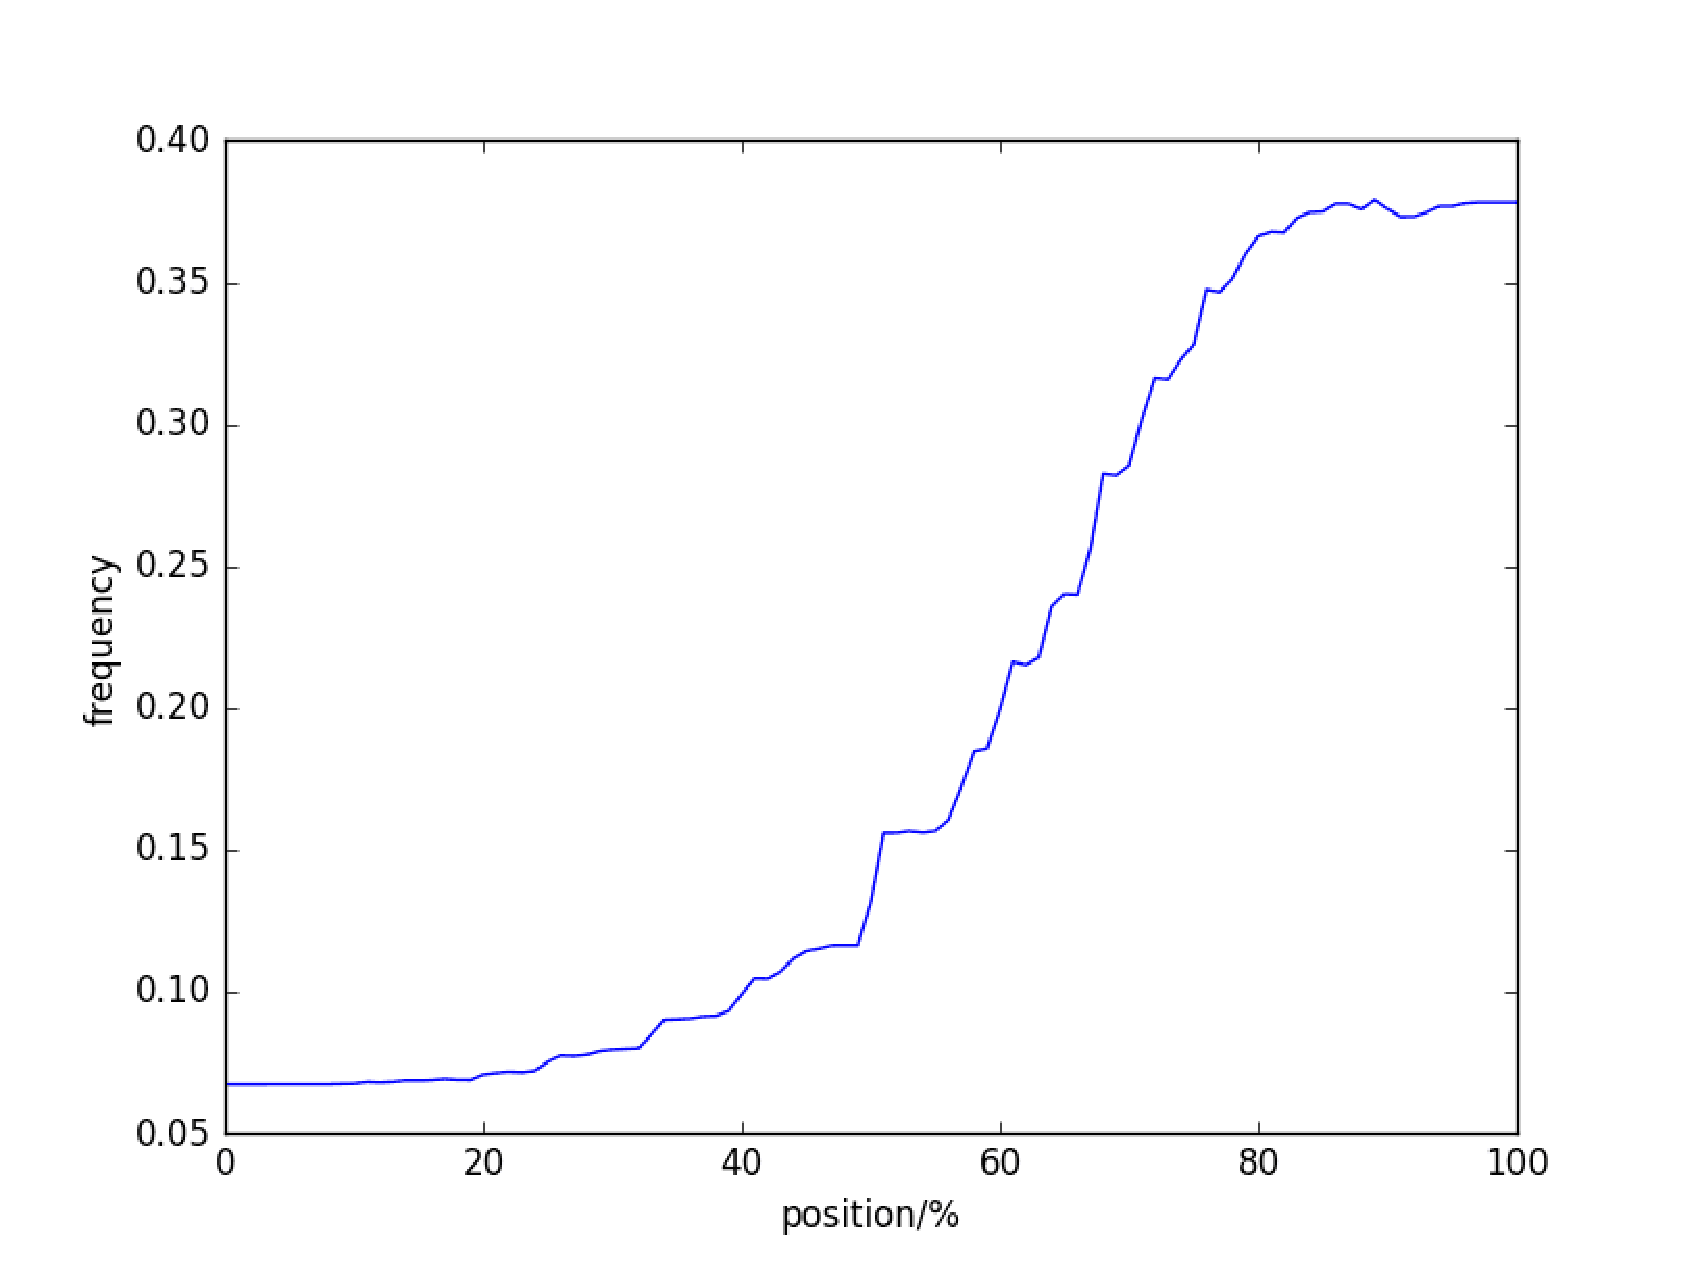
\includegraphics[width=2in]{figures/word_position.eps}
% \caption{Similar to \ref{fig:character_position}, this figure shows the relationship between the position of the overlapped words in question sentences and the occurrence frenquency of correct answers.}
% \label{fig:word_position}
% \end{figure}



%It is obvious that the overlapped characters(words) which often appear in the back of one sentence tends to be more important for us to find out the correct answer among answer text sets. We can also conclude from the two figures above that keywords or characters are more likely to appear in the back of the question sentences. Thus, we should give them higher weight than the rest.
%Unforturnatly, word-overlap based method is still based on the hypothesis of word independence. Synonym rewriting based methods and translation model could model words which are extremely closed in meaning to some extent. To enumerate a rewriting templet(translate templet) of high quality and maturity is never a easy task. Current embedding methods, to some degree, model this kind of semantic similarity from semantic space of high dimensional, which will be analysed in Sec~\ref{sec:embedding}.
%In Chinese, word group is composed of more Fined-grained characters. And word based overlap is a crude method to consider the correlation between words, which can be combined with other methods.


\subsection{Data Preprocessing}
\label{sec:preprocess}

Due to the lack of the obvious boundaries of Chinese text, we use the pynlpir package \footnote{https://github.com/tsroten/pynlpir} \cite{Liu2010Language} to segment both the question sentences and the answer texts. Stopwords \footnote{stopwords in http://tcci.ccf.org.cn/conference/2016/pages/page05\_evadata.html} are removed for dropping the useless high-frequency words which are not discriminative and have little semantic meaning. In order to get the classfication information of answer, we adopt the LTP online API \footnote{http://www.ltp-cloud.com/} for Named Entity Recognition (NER). The 300-dimention word embedding is provided by the NLPCC competition. Moreover, we have trained {\color{red}an} embedding model of some crawled pages in Baidu Baike~\footnote{http://baike.baidu.com/}. 
%The NlPCC test have supplied a word vectors which have 300 
%Embeding some message please
\begin{figure}
\centering
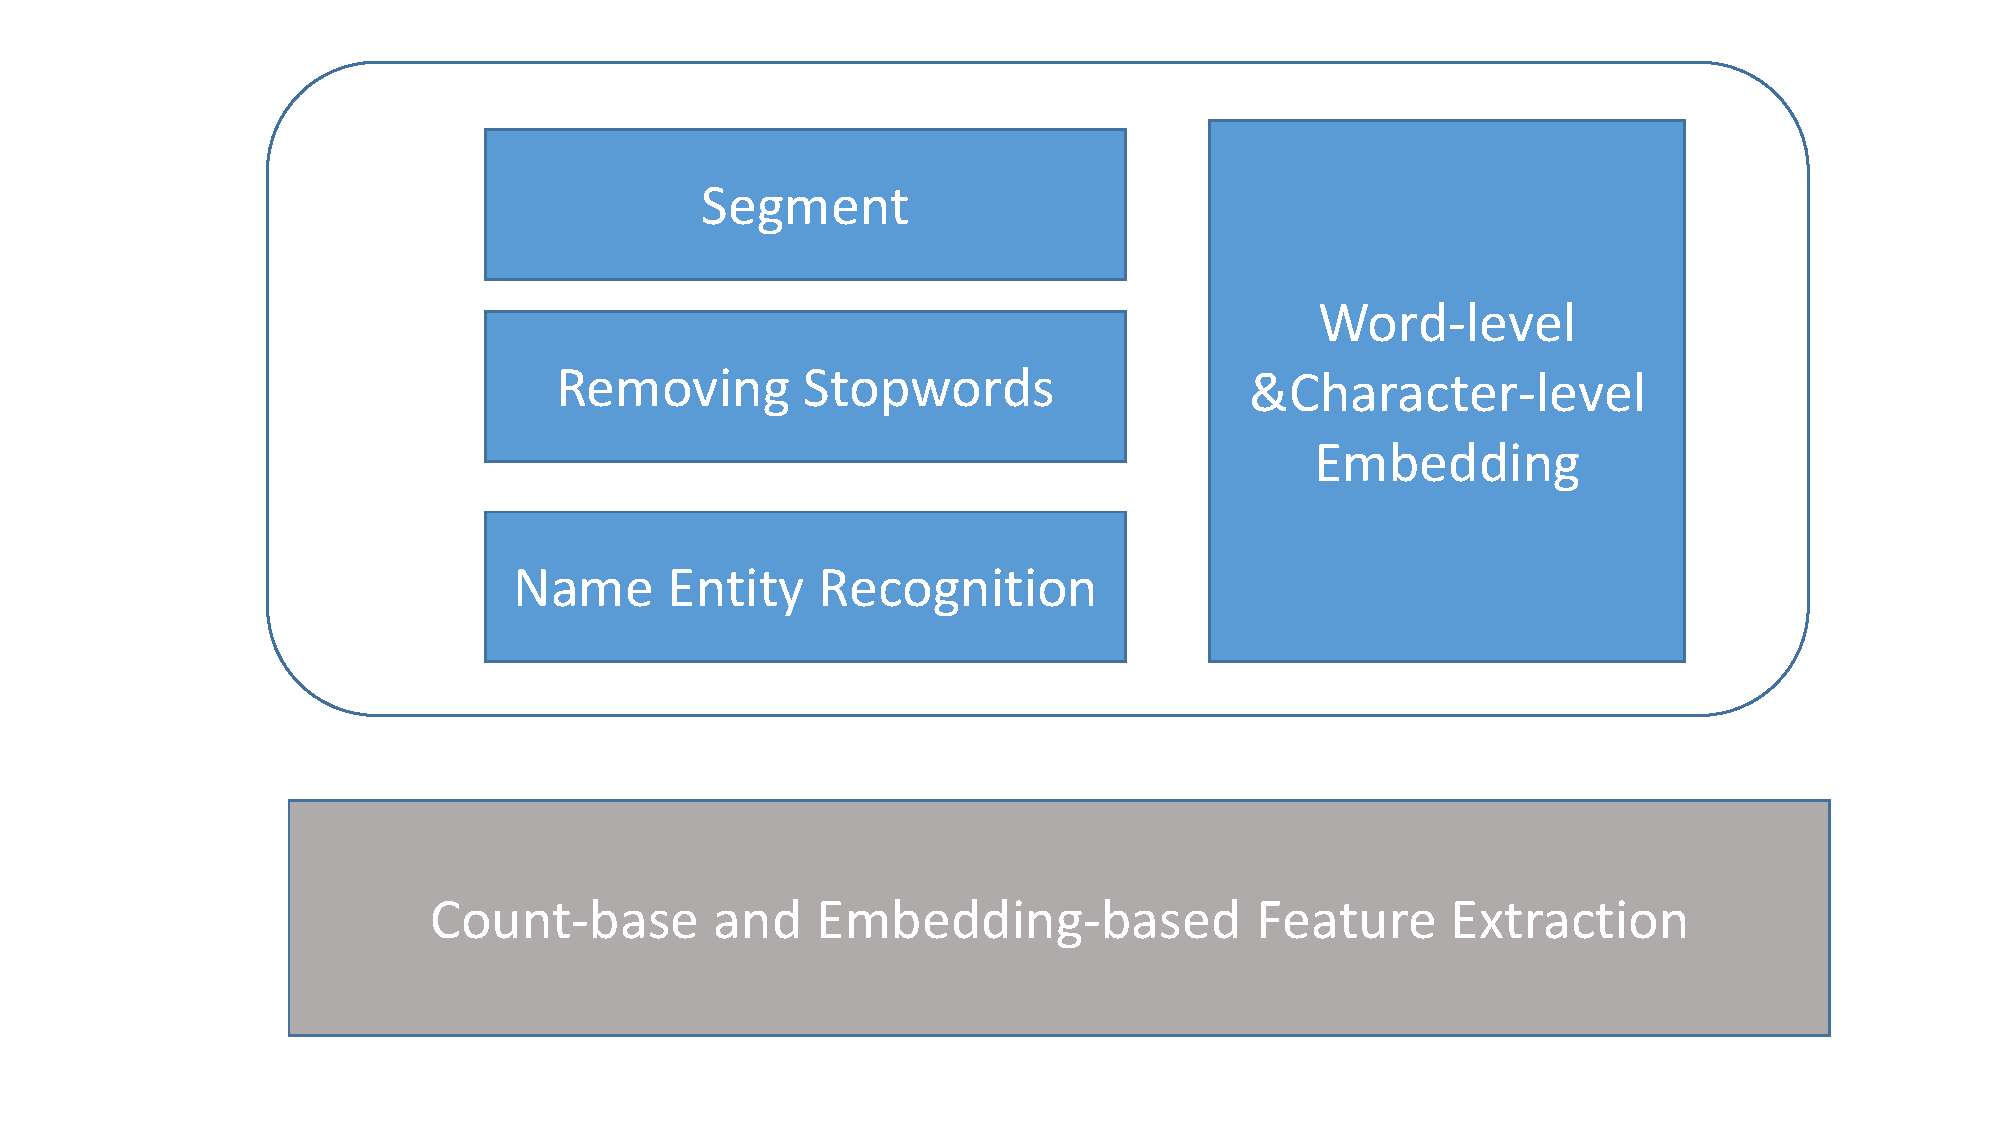
\includegraphics[width=12cm]{figures/structure.pdf}
\caption{the basic structure of the data prepare}
\label{fig:structure}
\end{figure}


%We uses the pynlpir package \footnote{http://github.com/tsroten} to segment both the question sentences and the answer texts into word groups and we base our next work on these words.We then omit some of the stop words like “的,是,在…”in those word groups according to the stop words list(http://).It is necessary to cut out several meaningless words since it is of great help to extracting the words overlap feature.Finally, we get a processed dataset of words.

% Other than the tranditional preprocess for Chinese text data, we try to expand some words to the original question for


\subsection{Feature Extraction}
\label{sec:feature}

\subsubsection{Questions' categories and Answers’ classfication}

As mentioned in the Sec.~\ref{sec:exploration}, 
%But if little information is mentioned in the sentence,it is certain that the sentence will never be the target answer.Therefore, the type information helps to classify questions and answers as well as find the target answers.
The questions can be divided into 5 categories. 3 of them are concerned with name entity, which are \emph{person}, \emph{place}, \emph{organization}. The  remaining two are \emph{time} and \emph{number}. Due to the lack of large-scale labeled datas, we can not adopt a learning-based question classifier~\cite{Li2003Learning}. Alternatively, a template-based question classifier can covers most cases for a simplified taxonomy. 
%However, we adopt the methods of extracting name entity to define the types of Person, Place and Organization and use model to find out the types of Time and Number because of the lack of supervised training and testing samples for learning. It turns out that our methods could cover more than 80\% cases and receive better results.
Answers' classfication may be a multilabeled task, which means an answer can belong to many categories. The first three NER-based categories can be recognized by the LTP online API. Meanwhile, we use templetes  of regular expression to distinguish the types of \emph{number} and \emph{time}. 

In practice, two methods are adopted. The first one is dummp Number, 5 categories are viewed as 5-dimention binary feature vectors {\color{red}whose} default value is unmatching. If the question is identified as one kind of category, the corresponding feature will be filled with matching {\color{red}flags}. 
The second {\color{red}method} is adopting one-dimention feature, which {\color{red}reflects whether} the category of question-answer pair matched or not.
% For each type, we use one-dimensional vector to indicate whether Question and Answer are matched or not.At the same time, or operation is made among the 5 types and the result is viewed as an one-dimensional vector for the reason that the result of each type is too sparse to count. The second method is that the answer texts which are well matched by keywords in the question are marked as “1” and those which are not matched are marked as “0”.


\subsubsection{Overlap}
%the count and position of overlap can    As QA pair match and Correlation have been mentioned in Sec~\ref{sec:exploration}, namely
In Sec~\ref{sec:exploration}, there are a{\color{red}kind of} statistical correlation between the matching probability and the overlapped information. 
%Specifically, the more words are overlapped in both question and answer sentences, the more likely that the answer is the target one. The
In these features, the {\color{red}deletion} of stop words seems to be vital due to the ignorance of the meaningless words. For Chinese text, it's hard for us to find the dictionay which can contain all the near-synonym pairs. An alternative approch is to use the charcter-based metric due to the fact that many synonymous paraphrased pairs share the same {\color{red}charcters in Chinese}. We calculate both the word-level and character-level scores of overlap as follows:
\begin{equation}
Score_{overlap}(Q,A)=\sum_{q_i \in Q}^n freq_{_A}(q_i)\cdot weight(q_i)  
\label{eq:overlap}
\end{equation}
Where the question sentence have $n$ words(characters) and the answer sentence have $m$ words(characters). The weighted model is based on the position of $q_j$ in the sentence. % and the IDF(inverse document frequency) of $q_j$ of the whole text collection.
$freq_{_A}(q_i)$ is denoted as the smoothed frequency of the $q_i$ in the answer $A$.
\subsubsection{TF-IDF model and BM25 model}
Some tranditional IR methods which are based on bag-of-words model are also implemented.

\begin{equation}
Score_{bm25}(Q,A)=\sum_{q_i \in Q}^nIDF(q_i)\cdot \frac{f_i\cdot(k_1+1)}{f_i + k_1 \cdot (1-b +b\cdot \frac{Length_A}{Lenght_{avg}})}  
\label{eq:bm25}
\end{equation}
where $f_i$ is the frequency of the $q_i$ in the answer $A$. $k_1$, b are parameters which can be {\color{red}adjusted} for the specific task. $Length_A$ and $Lenght_{avg}$ are the length of the answers $A$ and the average length of the whole answers.

\subsubsection{Other features}
Edit distance is usually used to measure the length of similar strings in English. While Jaccard index gives the similarity of morphemic sets between the questions and answers. The length of answer sentence is often considered as a significant feature.


\subsubsection{Embedding-based approach}
\label{sec:embedding}
Embedding technology embeds words into a high dimensional semantic space, which makes it easier to find the relationship between words. Sentence is simply considered to have been lapped by words linearly. Different words can contribute different weights for the whole meaning of a sentence, which depends on their position, semantic structure and IDF.
We get the representation of a word or Chinese character by the following approach.
\begin{equation}
Representation(S) = \frac{\sum_{i=0}^n weight(s_i)\cdot \overrightarrow { embedding(s_i)} }{\sum_{i=0}^n weight(s_i) }
\label{eq:representation}
\end{equation}
$s_i$ is the character or word in a sentence(question or answer), and $embedding(s_i)$ is the corresponding embedding vector. Then we calculate the inner product between the represention of question and answer as the final score.

Besides these linear combination of the inside word embedding, we have {\color{red}built} a CNN model to test how much the question-answer pair matches.
\begin{figure}
\centering
\includegraphics[width=16cm]{figures/model.eps}
\caption{ The picture need to be repainted}
\label{fig:model}
\end{figure}



\subsection{Model Selection}
\label{sec:model}
We have presented various fundamental features in last chapter, which will directly effect the degree of how question and answer matches. We adopt a linear regression model and learn-to-rank model \cite{Liu2009Learning} to integrate those features~\footnote{https://sourceforge.net/p/lemur/wiki/RankLib/}. While some ensemble learning methods like boosting and bagging models are also used.~\cite{Chen2016XGBoost} ~\footnote{http://xgboost.readthedocs.io/en/latest/}


\section{Results}
\label{sec:results}

\subsection{Dataset}

The provided datasets \footnote{ http://tcci.ccf.org.cn/conference/2016/pages/page05\_evadata.html} of the document-based quetion answer task contains a training data which have the label for the ground truth and a testing data which do not have the correct label. In the training dataset, each question has many candidate answers. The structure of the dataset can be illustrated by~Tab.\ref{tab:table1}, where 1 in the last column means the correct answer. The provided testing set only contains questions and their candidate answers. Each submission should only include a column of scores which will be evaluated by the evalutin toolkit.  


\begin{table}[!hbp]
\caption{Training Data Structure}
\scriptsize
\label{tab:table1}
\begin{tabular}{|l|l|c|}
 \hline
question & candidate answers & label \\ \hline
俄罗斯贝加尔湖的面积有多大?& 贝加尔湖是世界上最深和蓄水量最大的淡水湖。& 0 \\
\hline
俄罗斯贝加尔湖的面积有多大?& 它位于布里亚特共和国(Buryatiya)和伊尔库茨克州(Irkutsk)境内。&0\\
\hline
俄罗斯贝加尔湖的面积有多大?& 湖型狭长弯曲,宛如一弯新月,所以又有“月亮湖”之称。&0\\
\hline
俄罗斯贝加尔湖的面积有多大?& 贝加尔湖长636公里,平均宽48公里,最宽79.4公里,面积3.15万平方公里& 1\\
\hline
俄罗斯贝加尔湖的面积有多大?& 贝加尔湖湖水澄澈清冽,且稳定透明(透明度达40.8米),为世界第二。&0\\
\hline
\end{tabular}

\end{table}

\subsection{Evaluation Metrics}
Our Question Answering system will be evaluated by MRP and MAP. Mean Reciprocal Rank(MRR) mainly indicates that whether the recall results good or not depends on the rank of the correct answer, namely the higher the correct answer ranked, the better the results are.

\begin{equation}
MRR=\frac{1}{|Q|}\sum_{i=1}^{|Q|}\frac{1}{rank_{i}}
\end{equation}

$|Q|$ stands for the total number of questions in the evaluation set. For the \(i^{th}\) question \(Q_{i}\), \(rank_{i}\) represents the position of the first correct answer in the generated answer set \(C_{i}\).  \(\frac{1}{rank_{i}}\) equals 0, if \(C_{i}\) doesn't have the correspond answer with the golden answers \(A_{i}\) for \(Q_{i}\). 
%For example, if there are 4 queries in the test set. Suppose the correct answers for the first 3 queries are ranked 3,1,5 respectively and there is no answer for the last query.
%$$MRR=(\frac{1}{3}+\frac{1}{1}+\frac{1}{5}+0)\frac{1}{4}=0.383$$

Another evaluation metric is Mean Average Precision(MAP), which can be defined as follows.


\begin{equation}
MAP=\frac{1}{|Q|}\sum_{i=1}^{|Q|}AveP(C_{i},A_{i})   \
AveP(C,A)=\frac{\sum\nolimits_{k=1}^n(P(k)\cdot{rel(k)})}{min(m,n)}
\end{equation}

MAP mainly refers to the average precision of the results. If the correct anwser ranks high in the retrieved answer set, the value of MAP will also be high accordingly. $m$ denotes the number of correct answer sentences and $n$ is the number of retrieved answer sentences. $P(k)$ is the precision at cut-off k, which is the rank in the sequence of retrieved answer sentences. $rel(k)$ equals 1 if the item at rank k is an answer sentence, and 0 if not.


\subsection{Results}

The competition have provided four baselines as follows:%: \emph{Average Word Embeding}, \emph{Machine Translation} \emph{Paraphrase}, \emph{Word Overlap}. 
\begin{table}[!hbp]
\caption{the four baseline.}
\small % Font size can be changed to match table content. Recommend 10 pt by default.
\centering
\begin{tabular}{{p{6.5cm}p{3cm}p{3cm}}}
\toprule
\textbf{method}	& \textbf{MAP}	& \textbf{MRR}\\
\midrule
Average Word Embeding & 0.4610 & 0.4610 \\
Machine Translation & 0.2410 & 0.2412 \\
Paraphrase & 0.4886 &  0.4906\\
Word Overlap & 0.5114 & 0.5134 \\
\bottomrule
\end{tabular}
\label{fig:baselie}
\end{table}

Due to {\color{red}the fact} that the above methods are based on the bag-of-word model and do not have a learn-based mechanism, the performance is {\color{red}rather} poor. In our approach, we get the result as follow:

\begin{table}[!hbp]
\caption{our approach.}
\small % Font size can be changed to match table content. Recommend 10 pt by default.
\centering
\begin{tabular}{{p{6.5cm}p{3cm}p{3cm}}}
\toprule
\textbf{method}	& \textbf{MAP}	& \textbf{MRR}\\
\midrule
BM25 & 0.4610 & 0.4610 \\
weighted word overlap & 0.2410 & 0.2412 \\
weighted character overlap& 0.4886 &  0.4906\\
weighted word embedding & 0.5114 & 0.5134 \\
weighted character embedding & 0.5114 & 0.5134 \\
word-based NN & 0.5114 & 0.5134 \\
character-based NN & 0.5114 & 0.5134 \\
Emsenble learning of all features & 0.5114 & 0.5134 \\
\bottomrule
\end{tabular}
\label{fig:our_approach}
\end{table}
\subsection{discussion}

analsys our results

\section{Conclusion and Future Work}
\label{sec:discussion}
In this paper, we report technique details of our approach for the sub-task of NLPCC 2016 shared task Open Domain Question answering. Some traditional methods and neural-network based methods have been proposed. In our approach, we {\color{red}combine} the characters of Chinese text with our models and achieve a good performance by a emsenble learning strategy. 
In our opinions, {\color{red}an} effective repersentation which contains the sequencial(or tree-based) information of short text and the corresponding effective semantic matching are the two key factors of the QA system. An end-to-end system which is specifically applicable for Chinese may be the trend for Chinese Question-Answering system.   
 
\cite{Li2015Component}





%
% ---- Bibliography ----
%
% \begin{thebibliography}{}
%
% \bibitem{Rodriguez.{2010}}
% Open Source Cloud Computing Tools: A Case Study with a Weather Application
% Rodriguez-Martinez, M.; Seguel, J.; Greer, M.
% Cloud Computing (CLOUD), 2010 IEEE 3rd International Conference on
% Year: 2010
\bibliography{nlpcc_qa}
\bibliographystyle{IEEEtran}

% \end{thebibliography}

\end{CJK}
\end{document}
